% ============================================================
%  Aligning Small LLMs with GRPO for Strict JSON Generation
%  Beamer presentation — Adapted to DL26 guidelines
%  9 main slides + backup slides for Q&A
%  Compile with: pdflatex slides.tex (×2 for TikZ)
% ============================================================

\documentclass[10pt, aspectratio=169]{beamer}

% ── Theme ────────────────────────────────────────────────
\usetheme{metropolis}
\usepackage{appendixnumberbeamer}

% ── Packages ─────────────────────────────────────────────
\usepackage{booktabs}
\usepackage{tabularx}
\usepackage{array}
\usepackage{xcolor}
\usepackage[T1]{fontenc}
\usepackage[sfdefault,scaled=.9]{FiraSans}
\usepackage[lining,scaled=.88]{FiraMono}
\usepackage{graphicx}
\usepackage{microtype}
\usepackage{tikz}
\usetikzlibrary{arrows.meta, positioning, calc, backgrounds, fadings, shadows.blur}
\usepackage[most]{tcolorbox}
\usepackage{fontawesome5}
\usepackage{multicol}
\usepackage{etoolbox}
\usepackage{colortbl}

% ── Colour palette ───────────────────────────────────────
\definecolor{navy}{HTML}{1B2A4A}
\definecolor{sky}{HTML}{0EA5E9}
\definecolor{offwhite}{HTML}{F8FAFC}
\definecolor{accent}{HTML}{10B981}
\definecolor{warn}{HTML}{EF4444}
\definecolor{gold}{HTML}{F59E0B}
\definecolor{mint}{HTML}{6EE7B7}
\definecolor{slate}{HTML}{64748B}
\definecolor{darkbg}{HTML}{0F172A}

% ── Metropolis colour overrides ──────────────────────────
\setbeamercolor{normal text}      {fg=navy,   bg=white}
\setbeamercolor{frametitle}       {bg=navy,   fg=white}
\setbeamercolor{title separator}  {fg=sky}
\setbeamercolor{progress bar}     {fg=sky,    bg=navy!40}
\setbeamercolor{alerted text}     {fg=sky}
\setbeamercolor{block title}      {bg=navy!10, fg=navy}
\setbeamercolor{block body}       {bg=navy!5}
\setbeamercolor{title}            {fg=white}
\setbeamercolor{subtitle}         {fg=sky!70!white}
\setbeamercolor{author}           {fg=white!90}
\setbeamercolor{date}             {fg=white!70}

% ── Metropolis options ───────────────────────────────────
\metroset{
  titleformat  = regular,
  progressbar  = frametitle,
  block        = fill,
  sectionpage  = none,
  numbering    = fraction,
}

% ── Custom tcolorbox styles ──────────────────────────────
\tcbset{
  insightbox/.style={
    enhanced, boxrule=0pt, frame hidden,
    borderline west={3pt}{0pt}{#1},
    colback=#1!5, coltext=navy,
    left=8pt, right=6pt, top=5pt, bottom=5pt,
    fonttitle=\small\bfseries, coltitle=navy,
    sharp corners=east, rounded corners=west,
    arc=2pt,
  },
  insightbox/.default={sky},
  metricbox/.style={
    enhanced, boxrule=0.5pt,
    colframe=navy!20, colback=white,
    coltext=navy, halign=center,
    top=6pt, bottom=6pt, left=8pt, right=8pt,
    drop fuzzy shadow=navy!15,
    arc=4pt,
  },
  codebox/.style={
    enhanced, boxrule=0pt, frame hidden,
    colback=darkbg, coltext=white,
    fontupper=\ttfamily\scriptsize,
    left=8pt, right=8pt, top=6pt, bottom=6pt,
    arc=3pt,
  },
}

% ── Helper commands ──────────────────────────────────────
\newcommand{\highlightnum}[2]{{\bfseries\color{#2}#1}}
\newcommand{\iconitem}[2]{\item[\textcolor{sky}{#1}] #2}

% ── Metadata ─────────────────────────────────────────────
\title{Aligning Small LLMs with GRPO\\[0.25em]for Strict JSON Generation}
\subtitle{Rule-Based Reward Optimization for Schema-Conformant Output}
\author{Giuseppe Bellamacina}
\date{2026}

% ============================================================
\begin{document}

% ══════════════════════════════════════════════════════════
%  SLIDE 1 — Title (Required: course, track, name, repo)
% ══════════════════════════════════════════════════════════
{
  \setbeamertemplate{headline}{}
  \setbeamertemplate{footline}{}
  \begin{frame}[plain]
    \begin{tikzpicture}[remember picture, overlay]
      % Gradient background
      \fill[left color=navy, right color=navy!85!sky]
        (current page.south west) rectangle (current page.north east);
      % Decorative circles
      \foreach \x/\y/\r/\o in {
        12/3.5/1.8/8, 14/1/1.2/6, 1.5/4/1.4/5,
        3/0.5/0.9/7, 13.5/4.5/0.7/4, 0.5/1.5/1.0/6%
      }{
        \fill[sky, opacity=0.0\o] (\x,\y) circle (\r);
      }
      % Geometric accent lines
      \draw[sky!40, line width=0.5pt] (0,2.8) -- (16,2.8);
      \draw[sky!25, line width=0.3pt] (0,2.6) -- (16,2.6);
    \end{tikzpicture}
    \vspace{0.4cm}
    \begin{center}
      {\footnotesize\color{white!70}Deep Learning: Advanced Models and Methods (DL26) \textbullet\ \textbf{G23}}\\[0.6em]
      {\LARGE\bfseries\color{white}\inserttitle}\\[0.4em]
      {\normalsize\color{sky!70!white}\insertsubtitle}\\[1.0em]
      {\small\color{white!90}\insertauthor}\\[0.8em]
      {\footnotesize\color{sky!60}\faGithub~~\texttt{github.com/GiuseppeBellamacina/GRPO-strict-generation}}
    \end{center}
  \end{frame}
}

% ══════════════════════════════════════════════════════════
%  SLIDE 2 — Hook: Small LLMs Fail at Structured Output
% ══════════════════════════════════════════════════════════
\begin{frame}{Small LLMs ($<$2B) Cannot Reliably Produce Valid JSON}
  \begin{columns}[T]
    \begin{column}{0.55\textwidth}
      \begin{itemize}
        \setlength\itemsep{0.7em}
        \item[\textcolor{warn}{\faTimesCircle}] \textbf{31–39\% Pass@1} for SmolLM2-135M
        \newline{\scriptsize(39\% No-Think, 31\% with Think prompting)}
        \item[\textcolor{warn}{\faTimesCircle}] Unclosed brackets, type violations,
              conversational filler mixed with output
        \item[\textcolor{sky}{\faAngleRight}] \textbf{Goal:} use GRPO with rule-based rewards
              to reach $>$90\% Pass@1 — no neural reward model
        \item[\textcolor{sky}{\faAngleRight}] \textbf{Dense, deterministic, interpretable} signal
              drives alignment on a single GPU
      \end{itemize}
    \end{column}
    \begin{column}{0.42\textwidth}
      \begin{tcolorbox}[codebox, title={\color{warn}\faTimesCircle~Typical failure}, fonttitle=\scriptsize\bfseries, coltitle=warn]
Sure! Here's the JSON you asked for:
\{
~~"name": "Alice",
~~"age": 30,
~~"skills": ["Python", "ML"
\}

\textcolor{warn}{// Missing ] and extra text}
      \end{tcolorbox}
      \vspace{0.4em}
      \begin{tcolorbox}[codebox, title={\color{accent}\faCheckCircle~Expected output}, fonttitle=\scriptsize\bfseries, coltitle=accent]
```json
\{"name": "Alice", "age": 30,
~~"skills": ["Python", "ML"]\}
```
      \end{tcolorbox}
    \end{column}
  \end{columns}
\end{frame}

% ══════════════════════════════════════════════════════════
%  SLIDE 3 — Context: Models & Dataset
% ══════════════════════════════════════════════════════════
\begin{frame}{5 Models (135M–2B), Synthetic Dataset, Single GPU}
  \begin{columns}[T]
    \begin{column}{0.52\textwidth}
      \rowcolors{2}{navy!4}{white}
      \renewcommand{\arraystretch}{1.4}
      \centering
      \footnotesize
      \begin{tabular}{@{}lrl@{}}
        \toprule
        \textbf{Model}         & \textbf{Params} & \textbf{Arch} \\
        \midrule
        SmolLM2-135M-Instruct  & 135M & LLaMA-like \\
        SmolLM2-360M-Instruct  & 360M & LLaMA-like \\
        Qwen2.5-0.5B-Instruct  & 0.5B & Qwen2.5 \\
        TinyLlama-1.1B-Chat    & 1.1B & LLaMA 2 \\
        Gemma-2-2B-it          &   2B & Gemma 2 \\
        \bottomrule
      \end{tabular}
      \vspace{0.5em}

      \begin{tcolorbox}[insightbox=navy, title={\small Dataset}]
        \small
        \textcolor{sky}{\faFile}~24 parametric templates (8/difficulty)\\[0.3em]
        \textcolor{sky}{\faLayerGroup}~4\,500 training samples\\[0.3em]
        \textcolor{sky}{\faChartBar}~300 eval (100 S / 100 M / 100 H)\\[0.3em]
        \textcolor{sky}{\faBan}~No ground-truth JSON — reward evaluates directly
      \end{tcolorbox}
    \end{column}
    \begin{column}{0.45\textwidth}
      \vspace{0.2em}
      \begin{tcolorbox}[insightbox=sky, title={\small Configuration}]
        \small
        \textcolor{sky}{\faHdd}~4-bit NF4 quantization\\[0.35em]
        \textcolor{sky}{\faSitemap}~LoRA $r{=}16$,\; $\alpha{=}32$\\[0.35em]
        \textcolor{sky}{\faMicrochip}~1$\times$ NVIDIA L40S (48\,GB)\\[0.35em]
        \textcolor{sky}{\faRedo}~2\,500 steps / model\\[0.35em]
        \textcolor{sky}{\faCog}~Paged AdamW 8-bit\\[0.35em]
        \textcolor{sky}{\faGraduationCap}~LR $5{\times}10^{-6}$, cosine
      \end{tcolorbox}
      \vspace{0.5em}
      \begin{tcolorbox}[insightbox=gold]
        \scriptsize\textbf{4 strategies tested:}\\[2pt]
        Think / No-Think $\times$ Standard / Curriculum\\[2pt]
        Identical hyperparameters across all models
      \end{tcolorbox}
    \end{column}
  \end{columns}
\end{frame}

% ══════════════════════════════════════════════════════════
%  SLIDE 4 — Method: GRPO Pipeline
% ══════════════════════════════════════════════════════════
\begin{frame}{GRPO: Group-Relative Advantage Eliminates the Critic}
  \centering
  \resizebox{\textwidth}{!}{%
  \begin{tikzpicture}[
    node distance=0cm and 0.7cm,
    box/.style={
      rectangle, rounded corners=6pt,
      minimum width=3.2cm, minimum height=1.6cm,
      text centered, inner sep=6pt, text width=3.1cm,
      draw=navy!60, thick,
      drop shadow={shadow xshift=1pt, shadow yshift=-1.5pt, opacity=0.25, fill=navy!40}
    },
    sbox/.style={
      rectangle, rounded corners=4pt,
      minimum width=1.6cm, minimum height=0.7cm,
      text centered, inner sep=3pt, text width=1.5cm,
      draw=sky!50, fill=sky!8, thick, font=\scriptsize
    },
    arr/.style={-{Stealth[length=7pt, width=5pt]}, line width=1.2pt, color=navy!80},
    sarr/.style={-{Stealth[length=5pt]}, thick, color=sky!70},
  ]
    % ── Main pipeline nodes ──────────────────────────────
    \node[box, top color=sky!12, bottom color=sky!3] (p)
      {\small\textbf{Prompt} $x$\\[4pt]
       \scriptsize sampled from dataset\\
       difficulty $d\in\{S,M,H\}$};

    \node[box, top color=navy!10, bottom color=navy!3, right=0.7cm of p] (g)
      {\small\textbf{Sample} $G{=}8$\\[4pt]
       \scriptsize $y_1,\dots,y_8\sim\pi_\theta(\cdot|x)$\\
       temp $T\in[0.6,\,0.8]$};

    \node[box, top color=sky!25, bottom color=sky!8, right=0.7cm of g] (r)
      {\small\textbf{Score} $r_i$\\[4pt]
       \scriptsize $r_i=\sum\nolimits_k w_k\,r_k(y_i)$\\
       7 additive components};

    \node[box, top color=navy!12, bottom color=navy!4, right=0.7cm of r] (a)
      {\small\textbf{Advantage} $\hat{A}_i$\\[4pt]
       \scriptsize $\hat{A}_i=\dfrac{r_i-\bar{r}_G}{\sigma_{r_G}}$\\[2pt]
       group-relative norm.};

    \node[box, top color=sky!18, bottom color=sky!5, right=0.7cm of a] (u)
      {\small\textbf{Update} $\pi_\theta$\\[4pt]
       \scriptsize $\mathcal{L}=\sum_i\hat{A}_i\log\pi_\theta(y_i|x)$\\
       $-\,\beta\,D_{\mathrm{KL}}$,\quad$\beta{=}0.04$};

    % ── Arrow labels ─────────────────────────────────────
    \draw[arr] (p) -- node[above,font=\tiny\bfseries,color=navy!70]{prompt} (g);
    \draw[arr] (g) -- node[above,font=\tiny\bfseries,color=navy!70]{$G$ completions} (r);
    \draw[arr] (r) -- node[above,font=\tiny\bfseries,color=navy!70]{$\{r_i\}$} (a);
    \draw[arr] (a) -- node[above,font=\tiny\bfseries,color=navy!70]{$\{\hat{A}_i\}$} (u);

    % ── Feedback loop ─────────────────────────────────────
    \draw[arr, dashed, color=navy!50, rounded corners=10pt]
      (u.south) -- ++(0,-0.85)
      -- node[below, font=\tiny\itshape, color=slate, pos=0.5]
         {updated $\pi_\theta$ becomes new reference}
      ($(p.south)+(0,-0.85)$) -- (p.south);

    % ── Reward component sub-boxes (below Score node) ─────
    \node[sbox, below=1.2cm of r, xshift=-3.8cm] (c1) {format\\$w{=}0.20$};
    \node[sbox, right=0.14cm of c1]               (c2) {validity\\$w{=}0.25$};
    \node[sbox, right=0.14cm of c2]               (c3) {schema\\$w{=}0.25$};
    \node[sbox, right=0.14cm of c3]               (c4) {trunc.\\$w{=}0.10$};
    \node[sbox, right=0.14cm of c4]               (c5) {repet.\\$w{=}0.10$};
    \node[sbox, right=0.14cm of c5]               (c6) {strict.\\$w{=}0.10$};

    % horizontal collector bar + single arrow to Score node
    \coordinate (left)  at (c1.north west);
    \coordinate (right) at (c6.north east);
    \coordinate (mid)   at ($(left)!0.5!(right)$);
    \draw[sarr, rounded corners=3pt]
      (left) -- (right)
      (mid)  -- (r.south);

  \end{tikzpicture}}
  \vspace{0.3em}

  \begin{tcolorbox}[insightbox=sky, width=0.85\textwidth]
    \small\textbf{Key idea:} No critic network needed. Advantages are computed \emph{within} each group of $G{=}8$ completions.
    Additive reward composition ensures gradient is always non-zero — avoids \alert{zero-advantage collapse}.
  \end{tcolorbox}
\end{frame}

% ══════════════════════════════════════════════════════════
%  SLIDE 5 — Method: Reward Design + Curriculum
% ══════════════════════════════════════════════════════════
\begin{frame}{7 Additive Rewards + 3-Stage Curriculum Prevent Collapse}
  \begin{columns}[T]
    \begin{column}{0.52\textwidth}
      \centering
      \scriptsize
      \rowcolors{2}{navy!4}{white}
      \renewcommand{\arraystretch}{1.35}
      \setlength\tabcolsep{4pt}
      \begin{tabularx}{\linewidth}{@{}l c c X@{}}
        \toprule
        \textbf{Component} & \textbf{Range} & \textbf{$w$} & \textbf{Measures} \\
        \midrule
        \textcolor{sky}{\faCode}~format     & $[0,1]$    & .20 & \texttt{```json```} fence \\
        \textcolor{accent}{\faCheck}~validity   & $[0,1]$    & .25 & JSON parseability \\
        \textcolor{gold}{\faSitemap}~schema     & $[0,1]$    & .25 & Keys, types, nesting \\
        \textcolor{warn}{\faTimes}~truncation & $[-1,1]$   & .10 & Unclosed braces \\
        \textcolor{slate}{\faRedo}~repetition & $[-1,1]$   & .10 & Token loops \\
        \textcolor{navy}{\faBan}~strictness & $[-1,1]$   & .10 & Extra text outside JSON \\
        \textcolor{navy}{\faBrain}~reasoning  & $[-0.5,1]$ & .25\textsuperscript{*} & \texttt{<think>} quality \\
        \bottomrule
      \end{tabularx}
      {\tiny\color{slate} *Think mode only; weight redistributed when off}
    \end{column}
    \begin{column}{0.45\textwidth}
      \vspace{0.2em}
      % ── Curriculum timeline ──
      \centering
      \resizebox{\columnwidth}{!}{%
      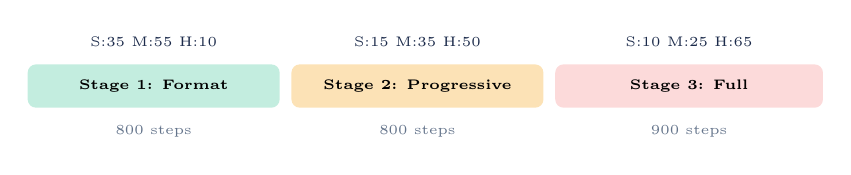
\begin{tikzpicture}
        % Stage bars
        \fill[accent!25, rounded corners=3pt] (0,0) rectangle (3.2,0.55);
        \fill[gold!30, rounded corners=3pt] (3.35,0) rectangle (6.55,0.55);
        \fill[warn!20, rounded corners=3pt] (6.7,0) rectangle (10.1,0.55);
        % Labels
        \node[font=\tiny\bfseries] at (1.6,0.28) {Stage 1: Format};
        \node[font=\tiny\bfseries] at (4.95,0.28) {Stage 2: Progressive};
        \node[font=\tiny\bfseries] at (8.4,0.28) {Stage 3: Full};
        % Steps
        \node[font=\tiny, color=slate, below=3pt] at (1.6,0) {800 steps};
        \node[font=\tiny, color=slate, below=3pt] at (4.95,0) {800 steps};
        \node[font=\tiny, color=slate, below=3pt] at (8.4,0) {900 steps};
        % Difficulty distribution
        \node[font=\tiny, color=navy, above=3pt] at (1.6,0.55) {S:35 M:55 H:10};
        \node[font=\tiny, color=navy, above=3pt] at (4.95,0.55) {S:15 M:35 H:50};
        \node[font=\tiny, color=navy, above=3pt] at (8.4,0.55) {S:10 M:25 H:65};
      \end{tikzpicture}}

      \vspace{0.8em}
      \begin{tcolorbox}[insightbox=accent]
        \scriptsize\textbf{Curriculum = safety net}\\[3pt]
        Prevents regression in strong models.\\
        Gemma-2-2B: $-$1.67pp (standard) $\to$ $+$0.67pp (curriculum)
      \end{tcolorbox}
      \vspace{0.3em}
      \begin{tcolorbox}[insightbox=sky]
        \scriptsize\textbf{Graduated partial credit}\\[3pt]
        Binary validity gives no gradient for near-valid JSON.
        Position-based scoring (0.20--0.70) keeps learning alive.
      \end{tcolorbox}
    \end{column}
  \end{columns}
\end{frame}

% ══════════════════════════════════════════════════════════
%  SLIDE 6 — Results: All Models Converge to 87–99%
% ══════════════════════════════════════════════════════════
\begin{frame}{All 5 Models Converge to 87–99\% Pass@1 After 2\,500 Steps}
  \centering
  \footnotesize
  \rowcolors{2}{navy!4}{white}
  \renewcommand{\arraystretch}{1.6}
  \setlength\tabcolsep{6pt}
  \begin{tabular}{@{}lcclc@{}}
    \toprule
    \textbf{Model} & \textbf{Pre} & \textbf{Peak} & \textbf{Best Configuration} & $\boldsymbol{\Delta}$ \\
    \midrule
    SmolLM2-135M   & 31\% & \textbf{90.00\%} & Think / Standard &  \highlightnum{+58.67 pp}{accent} \\
    SmolLM2-360M   & 78\% & \textbf{96.67\%} & No-Think / Standard &  \highlightnum{+19.00 pp}{accent} \\
    Qwen2.5-0.5B   & 92\% & \textbf{98.00\%} & Think / Curriculum &  \highlightnum{+6.33 pp}{accent} \\
    TinyLlama-1.1B & 79\% & \textbf{99.33\%} & No-Think / Curriculum &  \highlightnum{+20.00 pp}{accent} \\
    Gemma-2-2B     & 96\% & \textbf{97.67\%} & Think / Curriculum &  \highlightnum{+1.33 pp}{accent} \\
    \bottomrule
  \end{tabular}

  \vspace{0.5em}
  {\scriptsize\color{slate} All 5 models, best configuration per model. Pre = same-config baseline (Think lowers small-model baselines by $\sim$8pp).}

  \vspace{0.6em}
  \begin{columns}[T]
    \begin{column}{0.48\textwidth}
      \begin{tcolorbox}[metricbox]
        {\Large\bfseries\color{accent}+58.67 pp} {\normalsize largest gain}\\[2pt]
        {\scriptsize SmolLM2-135M: 31\% $\to$ 90\%}
      \end{tcolorbox}
    \end{column}
    \begin{column}{0.48\textwidth}
      \begin{tcolorbox}[metricbox]
        {\Large\bfseries\color{sky}99.33\%} {\normalsize best overall}\\[2pt]
        {\scriptsize TinyLlama-1.1B (No-Think / Curriculum)}
      \end{tcolorbox}
    \end{column}
  \end{columns}
\end{frame}

% ══════════════════════════════════════════════════════════
%  SLIDE 7 — Failure Case: Gemma U-Shaped Collapse
% ══════════════════════════════════════════════════════════
\begin{frame}{Gemma-2-2B Temporarily Collapses: Curriculum Pacing Must Match Capacity}
  \begin{columns}[c]
    \begin{column}{0.68\textwidth}
      \centering
      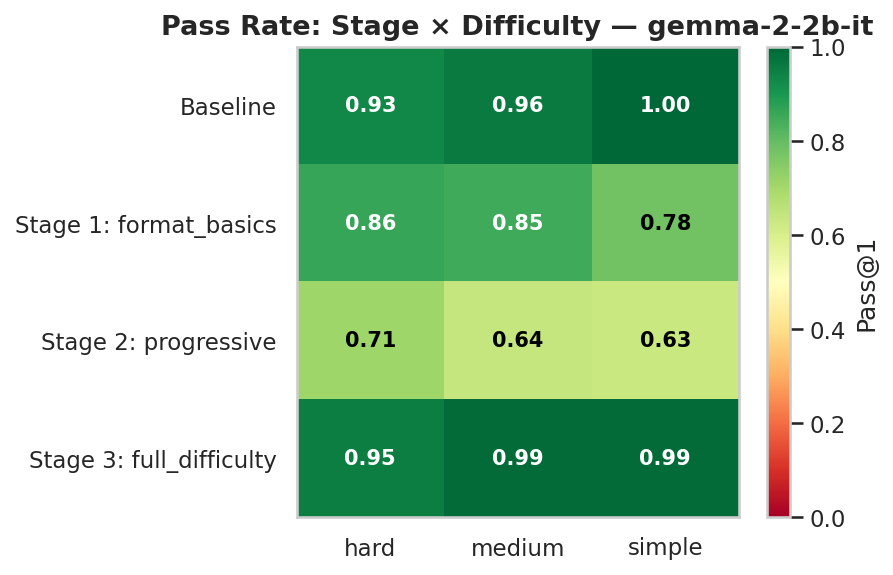
\includegraphics[width=\linewidth]{../../experiments/logs/grpo/think/curriculum/gemma2-2b/eval_20260413_030321/figures/stage_difficulty_heatmap.png}
      \\[0.3em]
      {\scriptsize\color{slate} Gemma-2-2B \textbullet\ Think / Curriculum \textbullet\ Pass@1 per stage \& difficulty}
    \end{column}
    \begin{column}{0.29\textwidth}
      \begin{tcolorbox}[insightbox=warn]
        \scriptsize\textbf{U-shaped collapse}\\[3pt]
        96\% $\to$ \textcolor{warn}{83\%} $\to$ \textcolor{warn}{66\%} $\to$ \textcolor{accent}{98\%}\\[4pt]
        Forcing \texttt{<think>} on trivial schemas confuses an already-strong model.\\[3pt]
        Full recovery only once hard schemas dominate (Stage 3).
      \end{tcolorbox}
      \vspace{0.5em}
      \begin{tcolorbox}[insightbox=accent]
        \scriptsize\textbf{Lesson}\\[3pt]
        Strong models need less warm-up.\\
        Standard training causes $-$1.67pp regression; Curriculum recovers to $+$0.67pp.
      \end{tcolorbox}
    \end{column}
  \end{columns}
\end{frame}

% ══════════════════════════════════════════════════════════
%  SLIDE 8 — Failure Analysis: How Errors Disappear
% ══════════════════════════════════════════════════════════
\begin{frame}{Errors Vanish Stage by Stage: Format First, Then Structure}
  \begin{columns}[c]
    \begin{column}{0.72\textwidth}
      \centering
      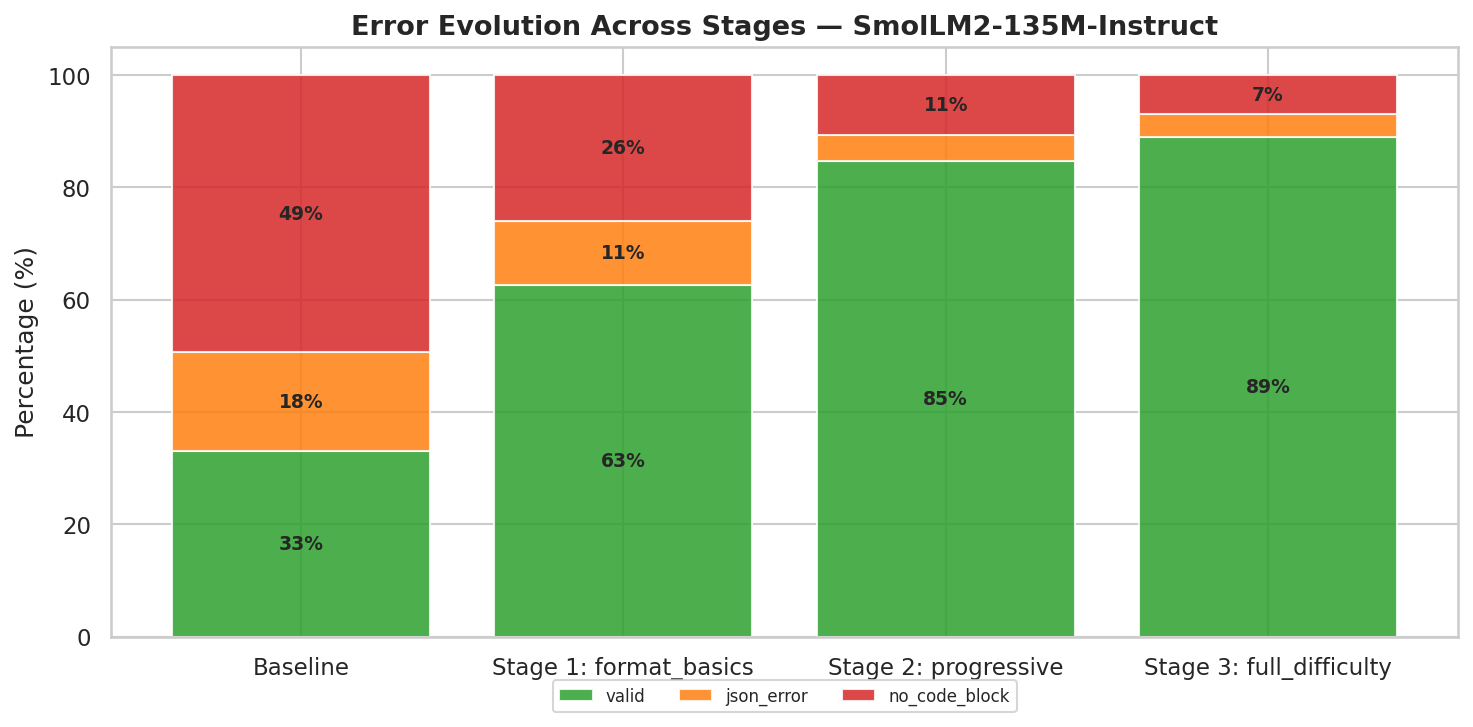
\includegraphics[width=\linewidth]{../../experiments/logs/grpo/nothink/curriculum/smollm2-135m/eval_20260410_060558/figures/error_evolution.png}
      \\[0.3em]
      {\scriptsize\color{slate} SmolLM2-135M \textbullet\ No-Think / Curriculum \textbullet\ Error types per stage}
    \end{column}
    \begin{column}{0.25\textwidth}
      \begin{tcolorbox}[insightbox=sky]
        \scriptsize\textbf{Stage 1}\\[2pt]
        Dominant error:\\\texttt{no\_code\_block}\\[2pt]
        Model learns the\\\texttt{```json```} fence first
      \end{tcolorbox}
      \vspace{0.3em}
      \begin{tcolorbox}[insightbox=gold]
        \scriptsize\textbf{Stage 2}\\[2pt]
        Format mastered.\\Residual: \texttt{json\_error}\\
        Focus shifts to structure
      \end{tcolorbox}
      \vspace{0.3em}
      \begin{tcolorbox}[insightbox=accent]
        \scriptsize\textbf{Stage 3}\\[2pt]
        Near-zero errors.\\Only edge-case\\schema failures remain
      \end{tcolorbox}
    \end{column}
  \end{columns}
\end{frame}

% ══════════════════════════════════════════════════════════
%  SLIDE 9 — Conclusions, Limits & Takeaways
% ══════════════════════════════════════════════════════════
\begin{frame}{Reward Design Matters More Than Model Size}
  \begin{columns}[T]
    \begin{column}{0.52\textwidth}
      \begin{tcolorbox}[insightbox=accent, title={\small Main Message}]
        \scriptsize
        GRPO with 7 additive rule-based rewards brings \textbf{all 5 models} (135M--2B) to \textbf{87--99\% Pass@1} on strict JSON generation, single GPU, identical hyperparameters.
      \end{tcolorbox}
      \vspace{0.3em}
      \begin{tcolorbox}[insightbox=sky, title={\small Takeaways}]
        \scriptsize
        \begin{enumerate}
          \setlength\itemsep{0.25em}
          \item \textbf{Standard} optimal for weak models (135M: +58.67pp)
          \item \textbf{Curriculum} safety net for strong models (prevents Gemma regression)
          \item \textbf{Think mode} $<$2pp marginal gain (small models can't produce \texttt{<think>})
        \end{enumerate}
      \end{tcolorbox}
    \end{column}
    \begin{column}{0.45\textwidth}
      \begin{tcolorbox}[insightbox=gold, title={\small Limitations}]
        \scriptsize
        \begin{itemize}
          \setlength\itemsep{0.2em}
          \item JSON-only — not directly generalizable
          \item Fully synthetic dataset; real-world gap unknown
          \item Fixed hyperparameters across models
        \end{itemize}
      \end{tcolorbox}
      \vspace{0.3em}
      \begin{tcolorbox}[insightbox=navy, title={\small Future Work}]
        \scriptsize
        \begin{itemize}
          \setlength\itemsep{0.2em}
          \item Extend to YAML, XML, SQL output
          \item Real-world API-call datasets
          \item Function reward ablation comparison
          \item Per-model hyperparameter tuning
        \end{itemize}
      \end{tcolorbox}
    \end{column}
  \end{columns}
\end{frame}

% ════════════════════════════════════════════════════════════
%  SLIDE 10 — Cross-Strategy Insights
% ════════════════════════════════════════════════════════════
\begin{frame}{Cross-Strategy Insights}
  \begin{columns}[T]
    \begin{column}{0.48\textwidth}
      \begin{tcolorbox}[insightbox=sky]
        \textcolor{sky}{\faBrain}~~\textbf{Think vs.\ No-Think}\\[3pt]
        \scriptsize Small models (135M, 360M, 0.5B) never generate \texttt{<think>} tokens;
        only Gemma and TinyLlama can.
        135M peaks 90\% in Think by exploiting other rewards, not reasoning.
      \end{tcolorbox}
      \vspace{0.4em}
      \begin{tcolorbox}[insightbox=accent]
        \textcolor{accent}{\faLock}~~\textbf{Curriculum = Safety Net}\\[3pt]
        \scriptsize Produces absolute highest scores (TinyLlama 99.33\%, Qwen 98.00\%).
        Standard causes Gemma to regress.
      \end{tcolorbox}
    \end{column}
    \begin{column}{0.48\textwidth}
      \begin{tcolorbox}[insightbox=gold]
        \textcolor{gold}{\faChartArea}~~\textbf{Inverted-U Gain Pattern}\\[3pt]
        \scriptsize Smallest models gain most: 135M $+$58pp.
        Mid-range: $+$13--26pp.
        Already-strong: $+$0--8pp (ceiling).
      \end{tcolorbox}
      \vspace{0.4em}
      \begin{tcolorbox}[insightbox=warn]
        \textcolor{warn}{\faExclamationTriangle}~~\textbf{Hard Tier Drives Improvement}\\[3pt]
        \scriptsize Baselines: 17--20\% hard pass for 135M.
        Post-GRPO: 86--99\% on hard prompts.
        Simple saturates to 100\% in Stage 1.
      \end{tcolorbox}
    \end{column}
  \end{columns}
\end{frame}

% ════════════════════════════════════════════════════════════
%  BACKUP SLIDES (for Q&A — not part of main presentation)
% ════════════════════════════════════════════════════════════
\appendix

{
  \setbeamertemplate{headline}{}
  \setbeamertemplate{footline}{}
  \begin{frame}[plain]
    \begin{tikzpicture}[remember picture, overlay]
      \fill[left color=navy, right color=darkbg]
        (current page.south west) rectangle (current page.north east);
    \end{tikzpicture}
    \vfill
    \begin{center}
      {\Huge\color{sky}\faFolderOpen}\\[0.8em]
      {\LARGE\bfseries\color{white}Backup Slides}\\[0.4em]
      {\small\color{white!60}Additional detail for Q\&A}
    \end{center}
    \vfill
  \end{frame}
}

% ── Backup: Baseline Detail ──────────────────────────────
\begin{frame}{Baseline Pass@1 — Per-Difficulty Breakdown}
  \centering
  \footnotesize
  \rowcolors{2}{navy!4}{white}
  \renewcommand{\arraystretch}{1.55}
  \setlength\tabcolsep{10pt}
  \begin{tabular}{@{}lcccc@{}}
    \toprule
    \textbf{Model} & \textbf{Overall} & \textbf{Simple} & \textbf{Medium} & \textbf{Hard} \\
    \midrule
    SmolLM2-135M   & 39.00\% & 58.00\% & 39.00\% & \textcolor{warn}{20.00\%} \\
    SmolLM2-360M   & 77.67\% & 85.00\% & 86.00\% & 62.00\% \\
    Qwen2.5-0.5B   & 92.67\% & 95.00\% & 95.00\% & 88.00\% \\
    TinyLlama-1.1B & 79.33\% & 89.00\% & 76.00\% & 73.00\% \\
    Gemma-2-2B     & \textbf{98.33\%} & \textbf{100\%} & \textbf{100\%} & \textbf{95.00\%} \\
    \bottomrule
  \end{tabular}

  \vspace{0.6em}
  {\scriptsize\color{slate} 300-sample balanced eval (100 S / 100 M / 100 H). Config: No-Think / Standard.}
\end{frame}

% ── Backup: Reward System Detail ─────────────────────────
\begin{frame}{Reward System — Full Think/No-Think Weight Table}
  \centering
  \scriptsize
  \rowcolors{2}{navy!4}{white}
  \renewcommand{\arraystretch}{1.4}
  \setlength\tabcolsep{5pt}
  \begin{tabularx}{0.99\linewidth}{@{}l c c c X@{}}
    \toprule
    \textbf{Component} & \textbf{Range} & \textbf{\,Think\,} & \textbf{\,NoThink\,} & \textbf{What it measures} \\
    \midrule
    \textcolor{sky}{\faCode}~\texttt{format}     & $[0,1]$      & 0.10 & 0.20 & \texttt{```json```} fence $\to$ 1.0 ~$\mid$~ generic fence $\to$ 0.5 ~$\mid$~ none $\to$ 0.0 \\
    \textcolor{accent}{\faCheck}~\texttt{validity}   & $[0,1]$      & 0.15 & 0.25 & JSON parseability; partial credit by error position (0.20--0.70) \\
    \textcolor{gold}{\faSitemap}~\texttt{schema}     & $[0,1]$      & 0.20 & 0.25 & Keys, types, nesting depth, required fields \\
    \textcolor{navy}{\faBrain}~\texttt{reasoning}  & $[-0.5,1]$   & 0.25 & \alert{0.0}  & \texttt{<think>} block quality; penalises missing/copied \\
    \textcolor{warn}{\faTimes}~\texttt{truncation} & $[-1,1]$     & 0.10 & 0.10 & Unclosed braces / unterminated strings \\
    \textcolor{slate}{\faRedo}~\texttt{repetition} & $[-1,1]$     & 0.10 & 0.10 & Token loops, repeated lines, duplicate blocks \\
    \textcolor{navy}{\faBan}~\texttt{strictness} & $[-1,1]$     & 0.10 & 0.10 & Extra text outside JSON $>$50\% of output \\
    \bottomrule
  \end{tabularx}
  \vspace{0.5em}

  \begin{tcolorbox}[insightbox=sky, width=0.85\textwidth]
    \small\textbf{Design principle:} Additive composition, no hard gating.
    Gradient is always non-zero; avoids \alert{zero-advantage collapse}.
    When Think is off, reasoning weight is redistributed proportionally.
  \end{tcolorbox}
\end{frame}

% ── Backup: SmolLM2-135M No-Think Standard ───────────────
\begin{frame}{SmolLM2-135M — No-Think / Standard Comparison}
  \centering
  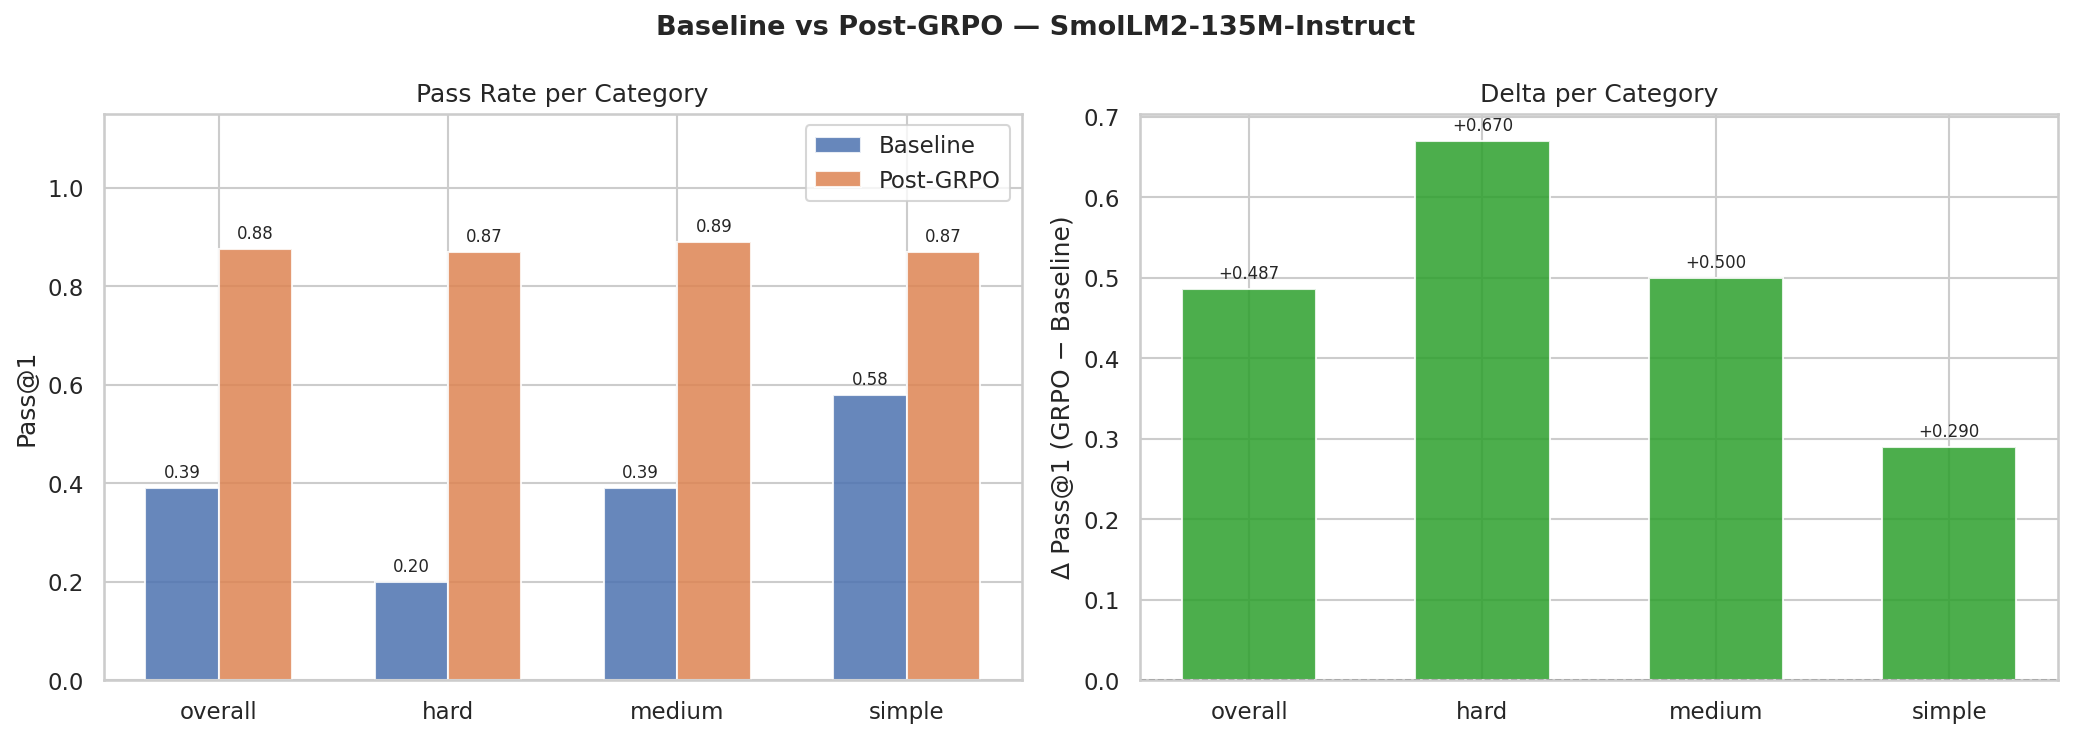
\includegraphics[width=0.78\linewidth]{../../experiments/logs/grpo/nothink/standard/smollm2-135m/eval_20260409_152243/figures/baseline_vs_grpo_comparison.png}
  \\[0.4em]
  {\small\color{slate} SmolLM2-135M \textbullet\ No-Think / Standard \textbullet\ Pass@1 by difficulty tier, baseline vs.\ GRPO}
\end{frame}

% ── Backup: Curriculum Progression (No-Think) ────────────
\begin{frame}{SmolLM2-135M — Curriculum Progression (No-Think)}
  \centering
  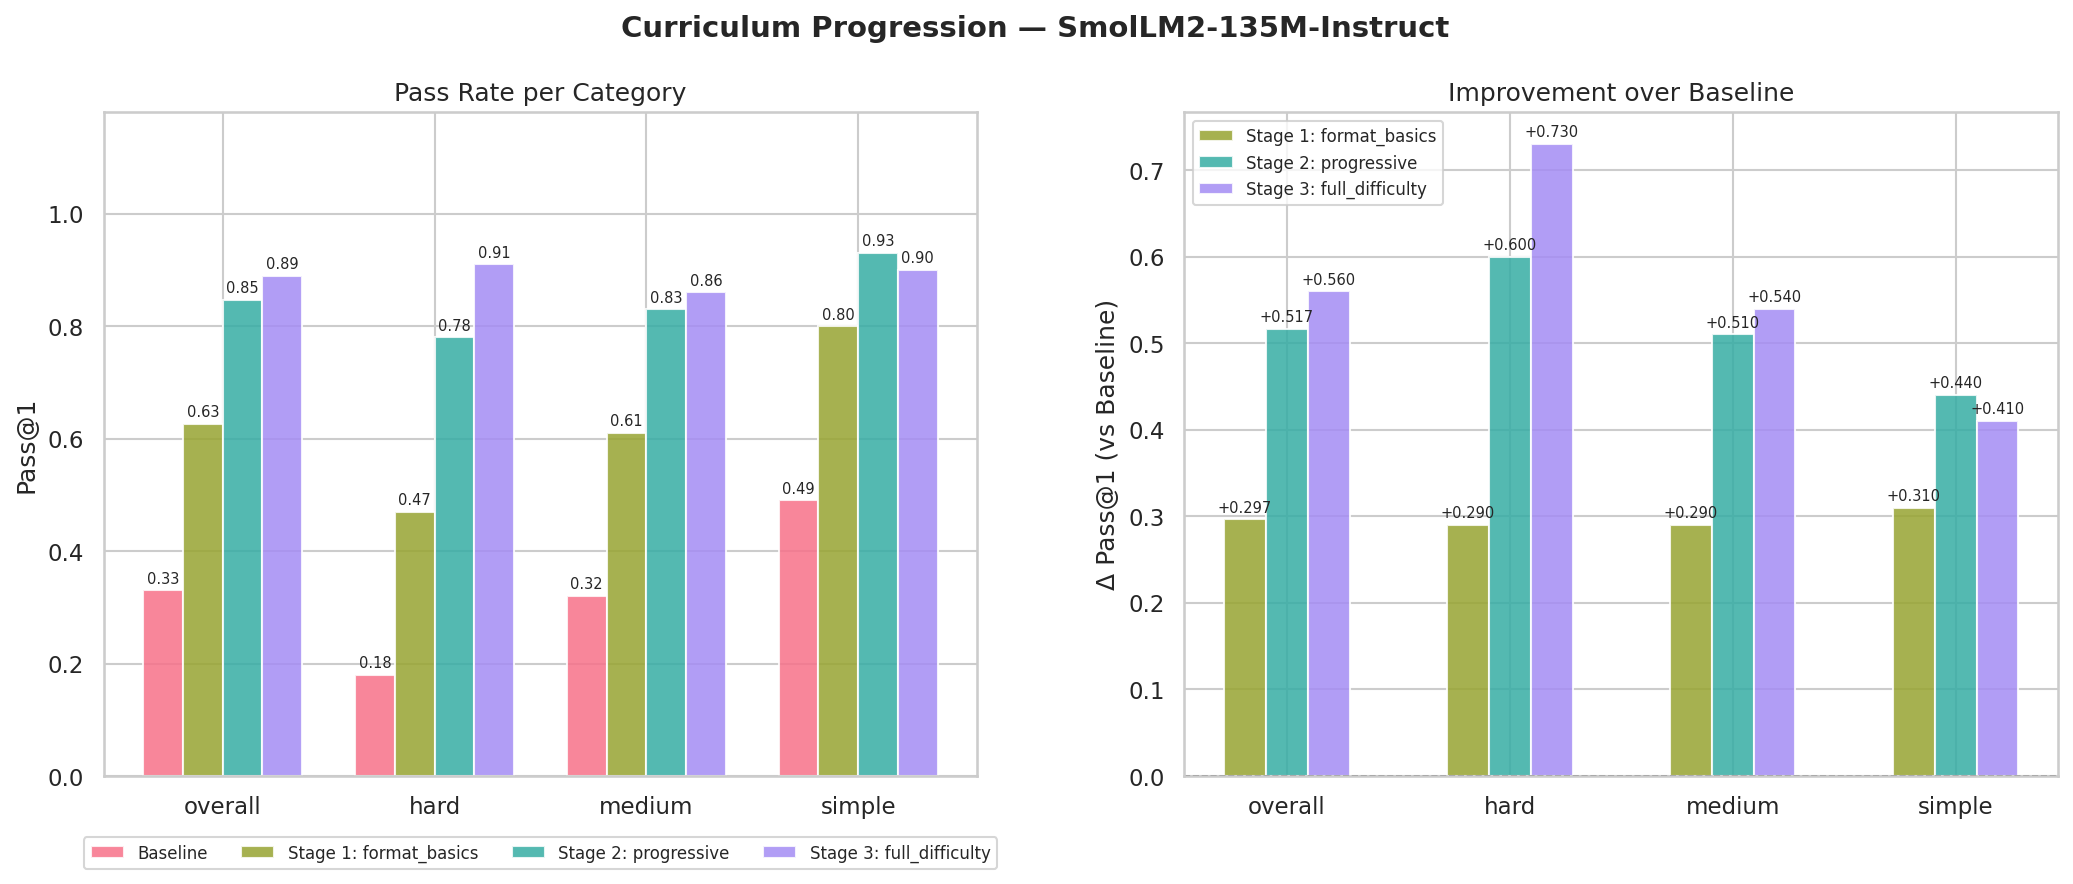
\includegraphics[width=0.78\linewidth]{../../experiments/logs/grpo/nothink/curriculum/smollm2-135m/eval_20260410_060558/figures/curriculum_progression.png}
  \\[0.4em]
  {\small\color{slate} SmolLM2-135M \textbullet\ No-Think / Curriculum \textbullet\ 33\% $\to$ 62.7\% $\to$ 84.7\% $\to$ 89.0\%}
\end{frame}

% ── Backup: Heatmap (No-Think / Curriculum) ──────────────
\begin{frame}{SmolLM2-135M — Difficulty Heatmap (No-Think / Curriculum)}
  \centering
  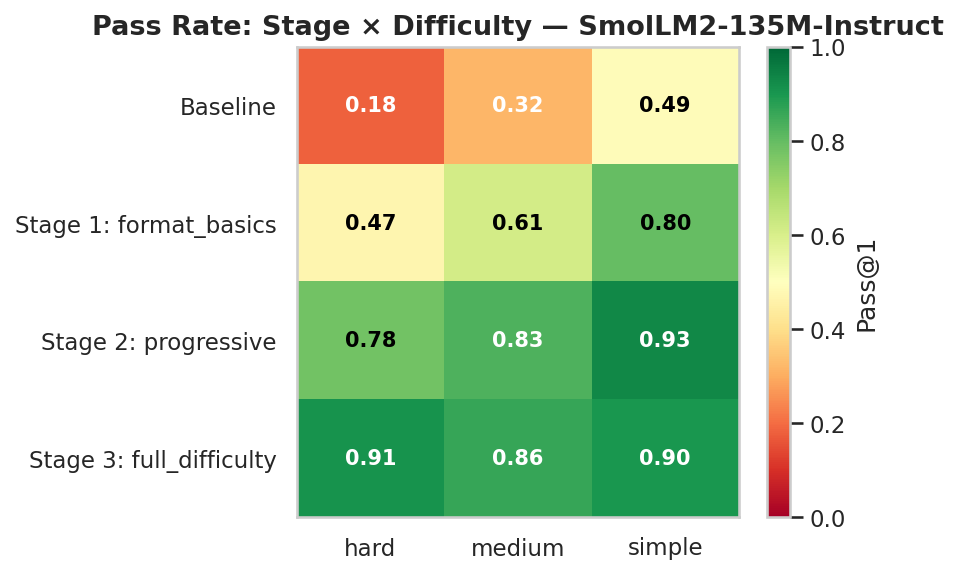
\includegraphics[width=0.78\linewidth]{../../experiments/logs/grpo/nothink/curriculum/smollm2-135m/eval_20260410_060558/figures/stage_difficulty_heatmap.png}
  \\[0.4em]
  {\small\color{slate} SmolLM2-135M \textbullet\ No-Think / Curriculum \textbullet\ Pass@1 per difficulty tier at each stage}
\end{frame}

% ── Backup: Curriculum Progression (Think) ───────────────
\begin{frame}{SmolLM2-135M — Curriculum Progression (Think)}
  \centering
  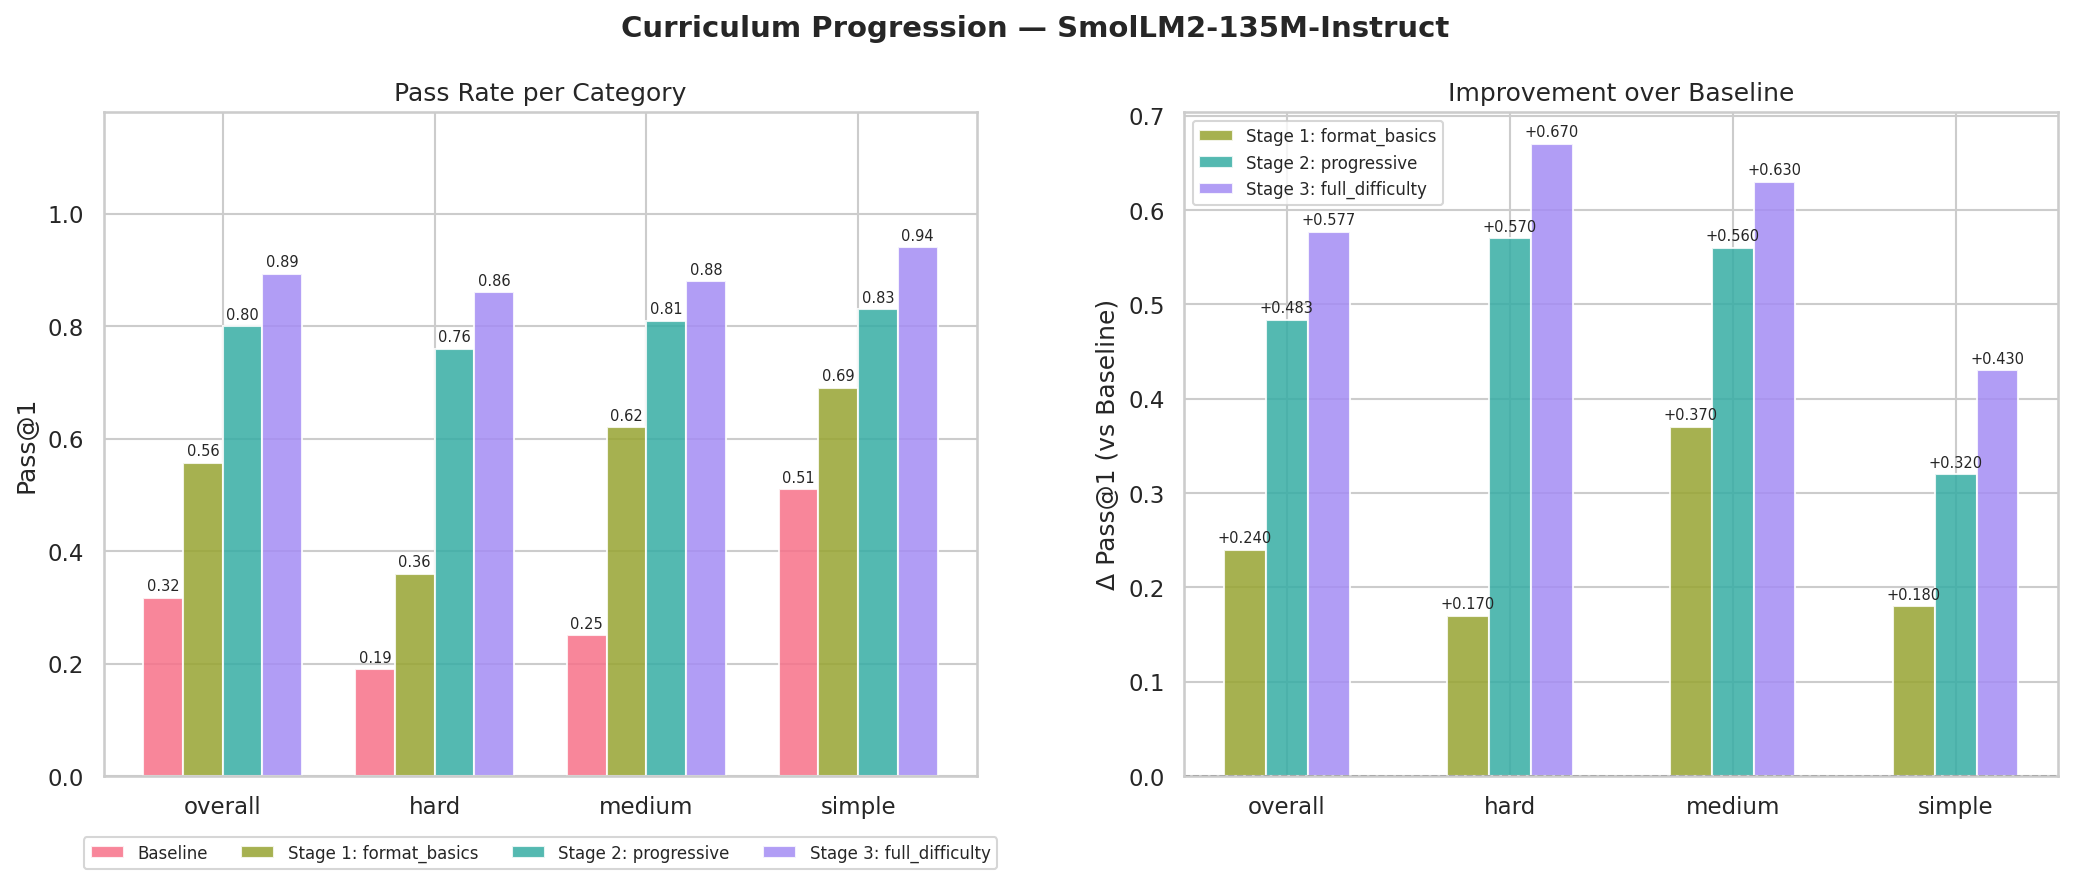
\includegraphics[width=0.78\linewidth]{../../experiments/logs/grpo/think/curriculum/smollm2-135m/eval_20260413_034728/figures/curriculum_progression.png}
  \\[0.4em]
  {\small\color{slate} SmolLM2-135M \textbullet\ Think / Curriculum \textbullet\ 31.7\% $\to$ 55.7\% $\to$ 80.0\% $\to$ 89.3\%}
\end{frame}

% ── Backup: Heatmap (Think / Curriculum) ─────────────────
\begin{frame}{SmolLM2-135M — Difficulty Heatmap (Think / Curriculum)}
  \centering
  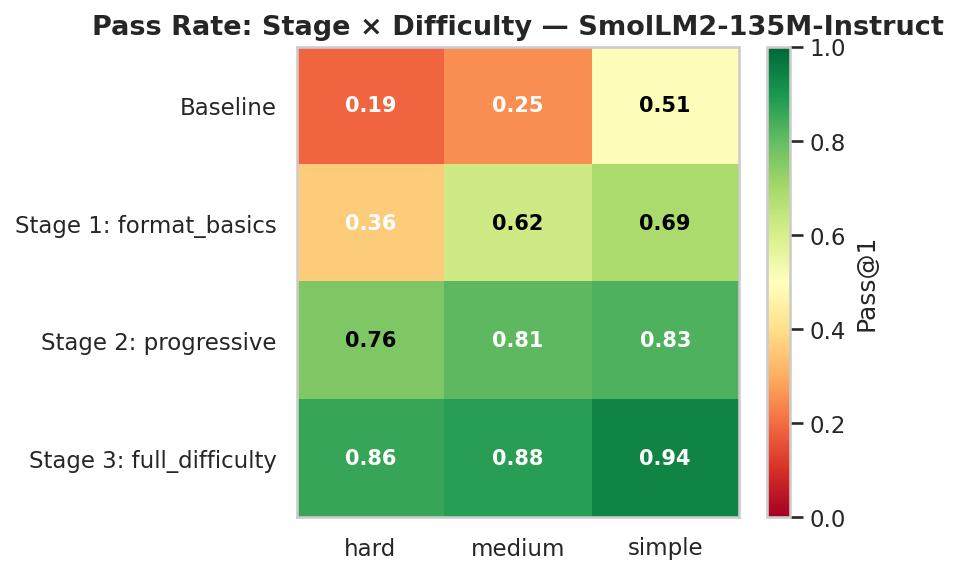
\includegraphics[width=0.78\linewidth]{../../experiments/logs/grpo/think/curriculum/smollm2-135m/eval_20260413_034728/figures/stage_difficulty_heatmap.png}
  \\[0.4em]
  {\small\color{slate} SmolLM2-135M \textbullet\ Think / Curriculum \textbullet\ Pass@1 per difficulty tier at each stage}
\end{frame}

% ── Backup: Reward Breakdown ─────────────────────────────
\begin{frame}{Reward Component Contributions at Final Checkpoint}
  \centering
  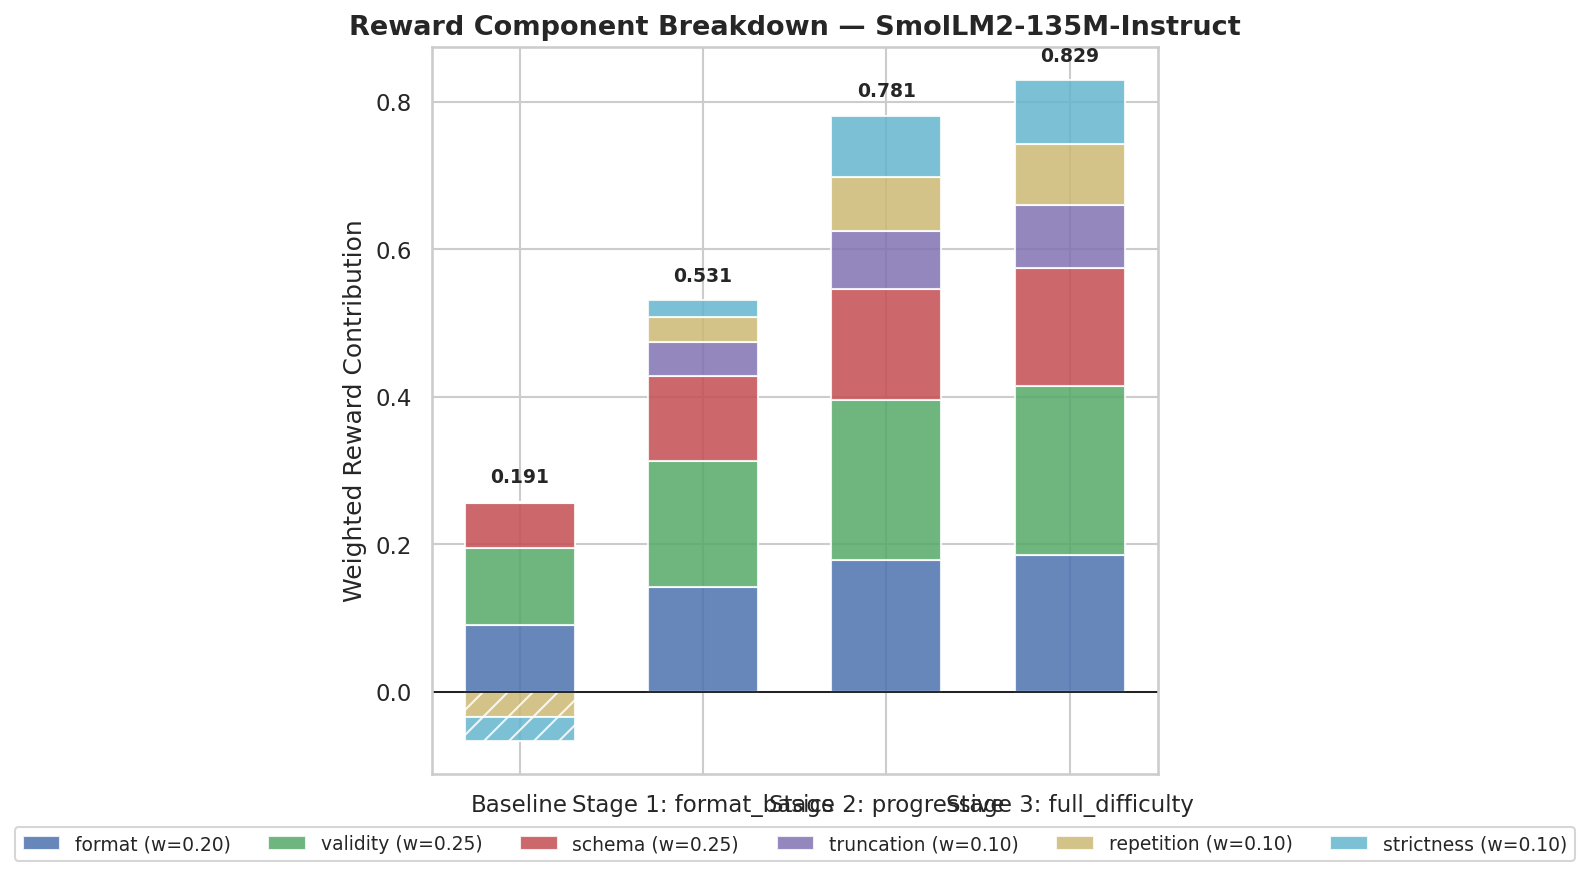
\includegraphics[width=0.80\linewidth]{../../experiments/logs/grpo/nothink/curriculum/smollm2-135m/eval_20260410_060558/figures/reward_breakdown.png}
  \\[0.4em]
  {\small\color{slate} SmolLM2-135M, No-Think / Curriculum}
\end{frame}

\end{document}
